
\begin{tabular}\href{https://assets.mozillalabs.com/Brands-Logos/Mozilla/mozilla_wordmark.png}{
\includegraphics{https://assets.mozillalabs.com/Brands-Logos/Mozilla/mozilla_wordmark.png}} \\ 
\textit{Community talk}\nolinebreakabout Mozilla by\nolinebreak\href{https://twitter.com/willyaranda}{Guillermo López}
\end{tabular}\href{http://www.mozilla.org/}{Mozilla foundation} is a huge community that involves different types of users and has a central message applied to all its levels:
\\
\\\textit{"Our mission is to promote openness, innovation \& opportunity on the Web."}\textit{
\\} In \href{http://www.mozilla.org/about/manifesto.html}{Mozilla Manifesto} you can read the whole document about freedom and accesibility that they apply day by day.

\subsubsection{ Brief History} The Foundation is consolidated by years of dedication to freedom of the web through its flagship Firefox. Since Netscape released the source code in 1998 Mozilla got down to work to develop a web browser from FLOSS source code they received from Netscape.
\\
\\ Mozilla wanted a free internet because IExplorer market share was 90\%. Was a private market and now this trend has changed.
\\
%  You may change the values of width and height above to resize the chart 

\\Source: \href{http://gs.statcounter.com/#browser-ww-yearly-2008-2013}{StatCounter Global Stats - Browser Market Share}
\\
\\ At last came out the first version of Firefox 0.6 on 6 December 2000. From here we have seen how the web has evolved at a breakneck speed of the hand of Firefox and other alternatives to IE.
\\
\\\textbf{Born in\nolinebreakJuly 15, 2003} with the \textit{leitmotiv}\nolinebreak"everyone can create their own content, \textit{create a participatory web}".\nolinebreak

\subsubsection{ Technologies} There is a bunch of technologies surrounding Mozilla development communities and of course, projects:
\\
\begin{itemize}
	\item \textit{Firefox} - Web Browser with a particularity that doesn't have portability to IOS because it uses Gecko instead of Webkit to render content. \nolinebreakApple doesn't allow a browser (or anyhting) that is not reder usgin Webkit.
	\item \textit{FirefoxOS} - New Mobile operative system based in HTML5 and Browser Oriented.
	\item \textit{Thunderbird} - eMail management but abandoned project. Developers have changed to Mozilla.
	\item \textit{Camino} - MacOS Mozilla Browser using Webkit
	\item \textit{Seamonkey} - Firefox, Thunderbird, Chat, Web Editor.
	\item \textit{Sundbird/Lightning} - Calendar project from Mozilla.
	\item \textit{XULRunner} - It's like Java Virtual Machine allowing multiplatform products oriented to Mozilla packages.
\end{itemize} And of course, developer tools to work with Mozilla community:
\begin{itemize}
	\item \textit{Mailing lists}\nolinebreak- For developers, information, everything related to \href{https://lists.mozilla.org/listinfo}{Mozilla}.
	\item \textit{Bug Tracking System}\nolinebreak-\nolinebreak\href{https://bugzilla.mozilla.org/}{Bugzilla}\nolinebreakfor every product.
\end{itemize}\href{http://2.bp.blogspot.com/-OGaTkm3Zijs/USd4Nuv3aOI/AAAAAAAADco/gHm17NaXbTc/s1600/bugzilla.png}{
\includegraphics{http://2.bp.blogspot.com/-OGaTkm3Zijs/USd4Nuv3aOI/AAAAAAAADco/gHm17NaXbTc/s320/bugzilla.png}}
\\
\begin{itemize}
	\item \textit{Source Code Managemet}\nolinebreak- Baazar, Mercurial, SVN, CVS.
	\item \textit{MXR}\nolinebreak- Cross references about the code from Mozilla (\href{http://mxr.mozilla.org/}{mxr}).
	\item \textit{Forge for scm}\nolinebreak- GitHub.
	\item \textit{QMO}\nolinebreak-\nolinebreakHome of Mozilla's testing and\nolinebreak\href{http://quality.mozilla.org/}{quality assurance community}.
	\item \textit{Cras Stats}\nolinebreak-\nolinebreak\href{http://graphs.mozilla.org/#displayrange=7&amp;branch=Firefox&amp;platform=%5B%22Windows+7%22%2C%22Windows+XP%22%2C%22Mac+OS+X%22%2C%22Linux%22%5D&amp;test=%5B%22Ts%22%2C%22Tp%22%2C%22SunSpider%22%5D}{Continuous integration}\nolinebreakserver output visualizations using\nolinebreak\href{https://github.com/mozilla/socorro}{Socorro}.
\end{itemize}\href{http://3.bp.blogspot.com/-UMzglU_lE3Q/USd4kABncMI/AAAAAAAADcw/Dmhpi_OESuQ/s1600/firefox-crash-reports.png}{
\includegraphics{http://3.bp.blogspot.com/-UMzglU_lE3Q/USd4kABncMI/AAAAAAAADcw/Dmhpi_OESuQ/s400/firefox-crash-reports.png}}
\\
\begin{itemize}
	\item \textit{Graph CI}\nolinebreak- Graphic visualization for every built from the code in\nolinebreak\href{http://graphs.mozilla.org/}{graph section}.
\end{itemize}\href{http://2.bp.blogspot.com/-YTH4s4enhL0/USd4oP1h0II/AAAAAAAADc4/zDljH9ycG5E/s1600/graphs-builds.png}{
\includegraphics{http://2.bp.blogspot.com/-YTH4s4enhL0/USd4oP1h0II/AAAAAAAADc4/zDljH9ycG5E/s640/graphs-builds.png}}
\\
\begin{itemize}
	\item \textit{Tinderbox}\nolinebreak- Tool to navigate through\nolinebreak\href{http://tinderbox.mozilla.org/showbuilds.cgi}{build logs and results}.
\end{itemize}

\subsubsection{ How to contribute} Mozilla community is very community, this statement may sound redundant, but would be an accurate definition. He moved away from the technology and developers as standard for any project.
\\
\begin{tabular}\href{http://3.bp.blogspot.com/-n1o6Iy9pFi8/USdxQSYTFGI/AAAAAAAADcg/Ens4tu2Ae54/s1600/mozilla-community-developers.png}{
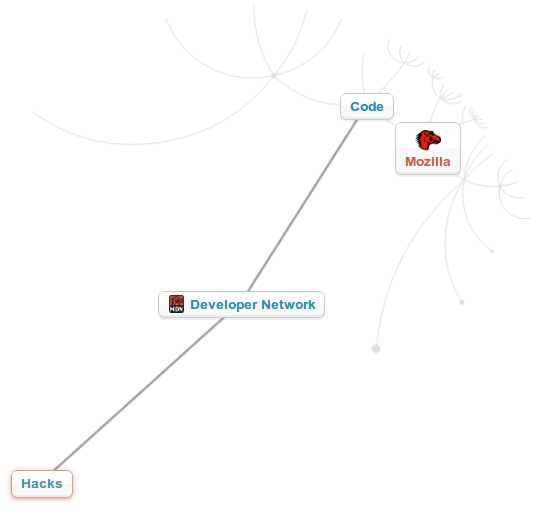
\includegraphics{http://3.bp.blogspot.com/-n1o6Iy9pFi8/USdxQSYTFGI/AAAAAAAADcg/Ens4tu2Ae54/s400/mozilla-community-developers.png}} \\ 
Mozilla developer community -\nolinebreak\href{http://www.mozilla.org/community/#hacks}{http://www.mozilla.org/community/}
\end{tabular} Mozilla has the basic steps as other FLOSS projects for \href{http://www.mozilla.org/es-ES/contribute/}{How to Contribute}\nolinebreakand gives you an oportunity to contribute in more than one way looking for a chance:
\\
\begin{itemize}
	\item Help for Users
	\item Quality control
	\item Programming
	\item Spread the word
	\item location
	\item Web Development
	\item Accessories
	\item graphic Design
	\item Documentation and drafting
	\item Education
\end{itemize} Furthermore gives you the oportunity to look for contribution near your location, a very useful tool. Mozilla invites you to be part of an Open Web. You don't have to be the smartest guy in the world they do this work spreading that all help is good an they will find for you the best place to help \textit{everyone}\nolinebreakwith your contribution.